% Options for packages loaded elsewhere
\PassOptionsToPackage{unicode}{hyperref}
\PassOptionsToPackage{hyphens}{url}
%
\documentclass[
]{article}
\usepackage{amsmath,amssymb}
\usepackage{iftex}
\ifPDFTeX
  \usepackage[T1]{fontenc}
  \usepackage[utf8]{inputenc}
  \usepackage{textcomp} % provide euro and other symbols
\else % if luatex or xetex
  \usepackage{unicode-math} % this also loads fontspec
  \defaultfontfeatures{Scale=MatchLowercase}
  \defaultfontfeatures[\rmfamily]{Ligatures=TeX,Scale=1}
\fi
\usepackage{lmodern}
\ifPDFTeX\else
  % xetex/luatex font selection
\fi
% Use upquote if available, for straight quotes in verbatim environments
\IfFileExists{upquote.sty}{\usepackage{upquote}}{}
\IfFileExists{microtype.sty}{% use microtype if available
  \usepackage[]{microtype}
  \UseMicrotypeSet[protrusion]{basicmath} % disable protrusion for tt fonts
}{}
\makeatletter
\@ifundefined{KOMAClassName}{% if non-KOMA class
  \IfFileExists{parskip.sty}{%
    \usepackage{parskip}
  }{% else
    \setlength{\parindent}{0pt}
    \setlength{\parskip}{6pt plus 2pt minus 1pt}}
}{% if KOMA class
  \KOMAoptions{parskip=half}}
\makeatother
\usepackage{xcolor}
\usepackage[margin=1in]{geometry}
\usepackage{graphicx}
\makeatletter
\def\maxwidth{\ifdim\Gin@nat@width>\linewidth\linewidth\else\Gin@nat@width\fi}
\def\maxheight{\ifdim\Gin@nat@height>\textheight\textheight\else\Gin@nat@height\fi}
\makeatother
% Scale images if necessary, so that they will not overflow the page
% margins by default, and it is still possible to overwrite the defaults
% using explicit options in \includegraphics[width, height, ...]{}
\setkeys{Gin}{width=\maxwidth,height=\maxheight,keepaspectratio}
% Set default figure placement to htbp
\makeatletter
\def\fps@figure{htbp}
\makeatother
\setlength{\emergencystretch}{3em} % prevent overfull lines
\providecommand{\tightlist}{%
  \setlength{\itemsep}{0pt}\setlength{\parskip}{0pt}}
\setcounter{secnumdepth}{-\maxdimen} % remove section numbering
\ifLuaTeX
  \usepackage{selnolig}  % disable illegal ligatures
\fi
\usepackage{bookmark}
\IfFileExists{xurl.sty}{\usepackage{xurl}}{} % add URL line breaks if available
\urlstyle{same}
\hypersetup{
  pdftitle={Summary report},
  hidelinks,
  pdfcreator={LaTeX via pandoc}}

\title{Summary report}
\author{}
\date{\vspace{-2.5em}2024-04-29}

\begin{document}
\maketitle

\section{Results for chromosome
NW\_022145594.1}\label{results-for-chromosome-nw_022145594.1}

\subsection{Local PCA outputs}\label{local-pca-outputs}

\begin{verbatim}
## [1] "Window type: snp Window size: 500"
## [1] "Window type: snp Window size: 1000"
## [1] "Window type: snp Window size: 5000"
## [1] "Window type: snp Window size: 10000"
\end{verbatim}

\includegraphics[width=1000px,height=300px]{lostruct_results/type_snp_size_500_chromosome_NW_022145594.1/figure/run_summary/plot_corners-1}
\includegraphics[width=1000px,height=300px]{lostruct_results/type_snp_size_1000_chromosome_NW_022145594.1/figure/run_summary/plot_corners-1}
\includegraphics[width=1000px,height=300px]{lostruct_results/type_snp_size_5000_chromosome_NW_022145594.1/figure/run_summary/plot_corners-1}
\includegraphics[width=1000px,height=300px]{lostruct_results/type_snp_size_10000_chromosome_NW_022145594.1/figure/run_summary/plot_corners-1}

\includegraphics[width=1000px,height=200px]{lostruct_results/type_snp_size_500_chromosome_NW_022145594.1/figure/run_summary/plot_corner_pca-1_1_2}
\includegraphics[width=1000px,height=200px]{lostruct_results/type_snp_size_1000_chromosome_NW_022145594.1/figure/run_summary/plot_corner_pca-1_1_2}
\includegraphics[width=1000px,height=200px]{lostruct_results/type_snp_size_5000_chromosome_NW_022145594.1/figure/run_summary/plot_corner_pca-1_1_2}
\includegraphics[width=1000px,height=200px]{lostruct_results/type_snp_size_10000_chromosome_NW_022145594.1/figure/run_summary/plot_corner_pca-1_1_2}

\subsection{Finding outlier regions}\label{finding-outlier-regions}

\includegraphics[width=1000px,height=800px]{outlier_regions_snp_chromosome_NW_022145594.1}

\end{document}
